% statistics_and_probability:x11 GDC:NO
\begin{question}
  \hspace*{\fill} [Note maximale: TBD]\par
  \medskip
  
  \noindent Un ensemble de données est: [\![ 18, 18, 19, 19, 20, 22, 22, 23, 27, 28, 28, 31, 34, 34, 36 ]\!]\par
  \noindent Le diagramme à boîtes et moustache de ces données est représenté ci-dessous.\par
  
  \medskip
  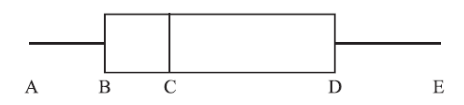
\includegraphics[scale=0.5]{boite_a_moustache_ensemble}\par  
  \medskip
  (a) Donnez les valeurs:\par
  \hspace{2em}$A =$\par
  \hspace{2em}$B =$\par
  \hspace{2em}$C =$\par
  \hspace{2em}$D =$\par
  \hspace{2em}$E =$\hspace*{\fill} [TBD]\par
  \medskip  
  (b) Trouvez l’intervalle interquartile.\hspace*{\fill} [TBD]\par
\end{question}

